%%
%% forked from https://gits-15.sys.kth.se/giampi/kthlatex kthlatex-0.2rc4 on 2020-02-13
%% expanded upon by Gerald Q. Maguire Jr.
%% This template has been adapted by Anders Sjögren to the University
%% Engineering Program in Computer Science at KTH ICT. Adaptation is the
%% translation of English headings into Swedish as the addition of Swedish
%% text. Original body text is deliberately left in English.


%% set the default lanage to english or swedish by passing an option to the documentclass - this handles the inside tile page
\documentclass[english, master]{tex/kththesis}
%\documentclass[swedish]{kththesis}

% \usepackage[style=numeric,sorting=none,backend=biber]{biblatex}

\setlength {\marginparwidth }{2cm} %leave some extra space for todo notes
\usepackage{todonotes}

\usepackage[perpage,para,symbol]{footmisc} %% use symbols to ``number'' footnotes and reset which symbol is used first on each page

%% Reduce hyphenation as much as possible
\hyphenpenalty=15000
\tolerance=1000
% include a variety of packages that are useful
%%----------------------------------------------------------------------------
%%   pcap2tex stuff
%%----------------------------------------------------------------------------
\usepackage{tikz}
\usetikzlibrary{arrows,decorations.pathmorphing,backgrounds,fit,positioning,calc,shapes}
\usepackage{pgfmath}	% --math engine

%% some additional useful packages
\usepackage{rotating}		%% For text rotating
\usepackage{array}		%% For table wrapping
\usepackage{graphicx}	        %% Support for images
\usepackage{float}		%% Suppor for more flexible floating box positioning
\usepackage{mdwlist}            %% various list-related commands
\usepackage{setspace}           %% For fine-grained control over line spacing
\usepackage{listings}		%% For source code listing
\usepackage{bytefield}          %% For packet drawings
\usepackage{tabularx}		%% For simple table stretching
\usepackage{multirow}	        %% Support for multirow colums in tables

\usepackage{url}                %% Support for breaking URLs
\usepackage{hyperref}
\usepackage[all]{hypcap}	%% prevents an issue related to hyperref and caption linking
%% setup hyperref to use the darkblue color on links
\hypersetup{colorlinks,breaklinks,
	linkcolor=darkblue,urlcolor=darkblue,
	anchorcolor=darkblue,citecolor=darkblue,linktoc=all}
% colorlinks=false, %set true if you want colored links

%% Some definitions of used colors
\definecolor{darkblue}{rgb}{0.0,0.0,0.3} %% define a color called darkblue
\definecolor{darkred}{rgb}{0.4,0.0,0.0}
\definecolor{red}{rgb}{0.7,0.0,0.0}
\definecolor{lightgrey}{rgb}{0.8,0.8,0.8}
\definecolor{grey}{rgb}{0.6,0.6,0.6}
\definecolor{darkgrey}{rgb}{0.4,0.4,0.4}
\definecolor{aqua}{rgb}{0.0, 1.0, 1.0}

%% If you are going to include source code (or code snippets)
\usepackage{listings}
%%\usepackage[cache=false]{minted} %% For source code highlighting
%%\usemintedstyle{borland}

\usepackage{csquotes} % Recommended by biblatex

% math stuff
\usepackage{amsmath}
\usepackage{amsthm}
\usepackage{amssymb}
\usepackage{xcolor}

\usepackage{subcaption}

% to correctly insert stressed characters
\usepackage[T1]{fontenc}
\usepackage[utf8]{inputenc}

% Add symbols
% \usepackage{textcomp}

% Code highlighting
% \usepackage{minted}
% \usemintedstyle{perldoc}
% \setminted{
%     frame=single,
%     breaklines,
% }

% Bibliography
% \usepackage[style=alphabetic]{biblatex}
% \usepackage[nottoc]{tocbibind}
% \usepackage{bibentry}
% \setcounter{biburllcpenalty}{9000}
% \usepackage{nameref}


%% Acronyms
% note that nonumberlist - removes the cross references to the pages where the acronym appears
% note that nomain - does not produce a main gloassay, this only acronyms will be in the glossary
% note that nopostdot - will present there being a period at the end of each entry
\usepackage[acronym, section=section, nonumberlist, nomain, nopostdot]{glossaries}
%\glsdisablehyper
\makeglossaries
% note the use of a non-breaking dash in the following acronym
% \newacronym{WiFi}{Wi-Fi}{Wireless Fidelity}

\newacronym{LP}{LP}{Linear Programming}
\newacronym{MIP}{MIP}{Mixed Integer Programming}
\newacronym{MILP}{MILP}{Mixed Integer Linear Programming}

\newacronym{DCS}{DCS}{Densest Common Subgraph}
\newacronym{BFF}{$\textsc{Bff}$}{Best Friends Forever}
\newacronym{O2BFF}{$\textsc{O}^{2} \textsc{Bff}$}{On-Off \acrshort{BFF}}

\newacronym{INCO}{INC$_{O}$}{\emph{Incremental overlap}}
                %load the acronyms file

%% definition of new command for bytefield package
\newcommand{\colorbitbox}[3]{%
	\rlap{\bitbox{#2}{\color{#1}\rule{\width}{\height}}}%
	\bitbox{#2}{#3}}

\newenvironment{swedishnotes}%
{\begin{center}
		\selectlanguage{swedish}
		\color{blue}}%
		{\end{center}\selectlanguage{english}
}

\begin{document}
\ifinswedish
	\selectlanguage{swedish}
\else
	\selectlanguage{english}
\fi


%% Information for inside title page
\title{This is the title in the language of the thesis}
\subtitle{A subtitle in the language of the thesis}

% give the alternative title - i.e., if the thesis is in English, then give a Swedish title
% \alttitle{Detta är den svenska översättningen av titeln}
% \altsubtitle{Detta är den svenska översättningen av undertiteln}
% alternative, if the thesis is in Swedish, then give an English title
%\alttitle{This is the English translation of the title}
%\altsubtitle{This is the English translation of the subtitle}

\authorsLastname{Zappia}
\authorsFirstname{Francesco}
\email{zappia@kth.se}
\kthid{u104906}
% If the student has an ORCiD - add it here
% \orcid{0000-0002-00001-1234}
\authorsSchool{\schoolAcronym{EECS}}

% If there is a second author - add them here:
% \secondAuthorsLastname{Student}
% \secondAuthorsFirstname{Fake B.}
% \secondemail{b@kth.se}
% \secondkthid{u100002}
% % If the student has an ORCiD - add it here
% \secondorcid{0000-0002-00001-5678}
% \secondAuthorsSchool{\schoolAcronym{ABE}}

\supervisorAsLastname{Neumann}
\supervisorAsFirstname{Stefan}
\supervisorAsEmail{neum@kth.se}
% If the supervisor is from within KTH add their KTHID, School and Department info
\supervisorAsKTHID{u112750}
\supervisorAsSchool{\schoolAcronym{EECS}}
\supervisorAsDepartment{Division of Theoretical Computer Science}
% other for a supervisor outside of KTH add their organization info
%\supervisorAsOrganization{Timbuktu University, Department of Pseudoscience}

%If there is a second supervisor add them here:
% \supervisorBsLastname{Supervisor}
% \supervisorBsFirstname{Another Busy}
% \supervisorBsEmail{sb@kth.se}
% % If the supervisor is from within KTH add their KTHID, School and Department info
% \supervisorBsKTHID{u100003}
% \supervisorBsSchool{\schoolAcronym{ABE}}
% \supervisorBsDepartment{Public Buildings}
% other for a supervisor outside of KTH add their organization info
%\supervisorBsOrganization{Timbuktu University, Department of Pseudoscience}

\examinersLastname{Gionis}
\examinersFirstname{Aristides}
\examinersEmail{argioni@kth.se}
% If the examiner is from within KTH add their KTHID, School and Department info
\examinersKTHID{u93105}
\examinersSchool{\schoolAcronym{EECS}}
\examinersDepartment{Division of Theoretical Computer Science}
% other for a examiner outside of KTH add their organization info
%\examinersOrganization{Timbuktu University, Department of Pseudoscience}


% \hostcompany{Företaget AB} % Remove this line if the project was not done at a host company
%\hostorganization{CERN}   % if there was a host organization

\date{\today}

\programcode{TCSCM}
%% Alternatively, you can say \programme{Civilingenjör Datateknik} to directly set the programme string

\titlepage
% document/book information page
\bookinfopage

% Frontmatter includes the abstracts and table-of-contents
\frontmatter
\setcounter{page}{1}

% \begin{abstract}
	\markboth{\abstractname}{}
	\todo[inline]{The first abstract should be in the language of the thesis.}
	\todo[inline, backgroundcolor=aqua]{Abstract fungerar på svenska också.}

	\todo[inline]{Keep in mind that most of your potential readers are only going to read your title and abstract. This is why it is important that the abstract give them enough information that they can decide is this document relevant to them or not. Otherwise the likely default choice is to ignore the rest of your document.\\
		A abstract should stand on its own, i.e., no citations, cross references to the body of the document, acronyms must be spelled out, …\\
		Write this early and revise as necessary. This will help keep you focused on what you are trying to do.}

	Write an abstract\todo{Use about 1/2 A4-page (250 and 350 words).}  with the following components:
	\begin{itemize}
		\item What is the topic area? (optional) Introduces the subject area for the project.
		\item Short problem statement
		\item Why was this problem worth a Master’s thesis project? (i.e., why is the problem both significant and of a suitable degree of difficulty for a Master’s thesis project? Why has no one else solved it yet?)
		\item How did you solve the problem? What was your method/insight?
		\item Results/Conclusions/Consequences/Impact: What are your key results/conclusions? What will others do based upon your results? What can be done now that you have finished - that could not be done before your thesis project was completed?\todo[inline]{The presentation of the results should be the main part of the abstract.}
	\end{itemize}

	\ifinswedish
		\subsection*{Nyckelord}
		5-6 nyckelord\todo{Nyckelord som beskriver innehållet i uppsatsrapporten}
	\else
		\subsection*{Keywords}
		5-6 keywords
	\fi
	\todo[inline]{Choosing good keywords can help others to locate your paper, thesis, dissertation, … and related work.}
	Choose the most specific keyword from those used in your domain, see for example:
	ACM's Computing Classification System (2012) or
	(2014) IEEE Taxonomy.

	Mechanics:
	\begin{itemize}
		\item The first letter of a keyword should be set with a capital letter and proper names should be capitalized as usual.
		\item Spell out acronyms and abbreviations.
		\item Avoid "stop words" - as they generally carry little or no information.
		\item List your keywords separated by commas (",").
	\end{itemize}
	Since you should have both English and Swedish keywords - you might think of ordering them in corresponding order (i.e., so that the nth word in each list correspond) - thus it would be easier to mechanically find matching keywords.


\end{abstract}
\cleardoublepage

\ifinswedish
	\selectlanguage{english}
\else
	\selectlanguage{swedish}
\fi
\begin{abstract}
	\markboth{\abstractname}{}
	\todo[inline]{All theses at KTH are required to have an abstract in both English and Swedish.\\
		If you are writing your thesis in English, you can leave this until the final version. If you are writing your thesis in Swedish then this should be done first – and you should revise as necessary along the way.\\
		If you are writing your thesis in English, then this section can be a summary targeted at a more general reader. However, if you are writing your thesis in Swedish, then the reverse is true – your abstract should be for your target audience, while an English summary can be written targeted at a more general audience.\\
		This means that the English abstract and Swedish sammnfattning
		or Swedish abstract and English summary need not be literal translations of each other.\\

		The abstract in the language used for the thesis should be the first abstract, while the Summary/Sammanfattning in the other language can follow.\\

		Exchange students many want to include one or more abstracts in the language(s) used in their home institutions to avoid the neeed to write another thesis when returing to their home institution.
	}

	\subsection*{Nyckelord}
	5-6 nyckelord\todo{Nyckelord som beskriver innehållet i uppsatsrapporten}


\end{abstract}

% \cleardoublepage
% \selectlanguage{italian} \todo[inline]{Use the relevant language for abstracts for your home university.\\
%     Note that you may need to augment the set of lanaguage used in polyglossia or
%     babel. The following languages represent the languages that have been used in
%     theses at KTH in 2018-2019, except for one in Chinese.
% }
% \begin{abstract}
%     \markboth{\abstractname}{}
%     Résumé en français
%
%     \subsection*{Mots clés}
%     5-6 mots-clés
% \end{abstract}
\cleardoublepage
% set to the language of the body of the thesis
\ifinswedish
	\selectlanguage{swedish}
\else
	\selectlanguage{english}
\fi

% \section*{Acknowledgments }
\markboth{Acknowledgments}{}

First of all I would like to deeply thank all that people helped me and gave me
suggestions during these months of research, motivating me as well as allowing me to
feel as one of their collegues: Dr. Stefan Neumann, my supervisor, Professor
Aristides Gionis, my examiner, and Professor Aris Anagnostopoulos, who joined us in this adventure.

I would also like to thank all my family and friends for supporting me through
all this years.

\bigskip
The computations were enabled by resources provided by the Swedish National Infrastructure for Computing
(SNIC) at the High Performance Computing Center North (HPC2N) partially funded by the Swedish Research Council through grant agreement no. 2018-05973.

This work has been developed as part of the SoBigData++ and REBOUND projects.
\acknowlegmentssignature


\fancypagestyle{plain}{}
\renewcommand{\chaptermark}[1]{ \markboth{#1}{}}
\tableofcontents
\markboth{\contentsname}{}

\cleardoublepage
\listoffigures

\cleardoublepage

\listoftables
\cleardoublepage
\listoflistings
\cleardoublepage
\printglossary[type=\acronymtype, title={List of acronyms and abbreviations}]
\todo[inline]{The list of acronyms and abbreviations should be in alphabetical
	order based on the spelling of the acronym or abbreviation.}


\label{pg:lastPageofPreface}
% Mainmatter is where the actual contents of the thesis goes
\mainmatter

\renewcommand{\chaptermark}[1]{\markboth{#1}{}}

% \chapter{Introduction}
\label{ch:introduction}

Social networks are nowadays largely used by people, allowing users to
interact and discuss the most different topics, but at the same time in these
platforms the polarization between users is constantly growing and several
studies have been conducted about it
\cite{Garimella2018}\cite{Guerra2013}\cite{conover2011political}\cite{gruzd2014investigating},
some of which focused on the recent debate about COVID-19
\cite{Jiang2021}\cite{green2020elusive}\cite{jiang2020political}\cite{lang2021maskon}
and vaccination \cite{Cossard2020}.

Polarization is the social phenomenon according to which people tend do
separate in opposing communities with few people remaining neutral
\cite{Guerra2013}. A close phenomenon is that of the Echo Chambers, groups in
which people that have the same opininions enforce their respective ideas
\cite{Garimella2018}, a concept very similar to the definition of polarization
as given in \cite{sunstein1999law}: ``group polarization arises when members of
a deliberating group move toward a more extreme point in whatever direction is
indicated by the members' predeliberation  tendency. `[L]ike polarized
molecules, group members become even more aligned in the direction they were
already tending.'\cite{turner1987rediscovering}''

In this document we aim at finding a method for finding Echo Chambers, by
analyzing data retrieved from social medias like Twitter and Reddit: we define
the \acrfull{ECP} and the \acrfull{D-ECP} and propose techniques for solving
and approximating them.

Both these $2$ problems are defined on a signed graph, i.e. distinguishing
between \emph{friendly} and \emph{hostyle} interactions between the users.
Differently from previous studies of polarization on signed graph
\cite{xiao2020searching}, we define
and incorporate in our problems the ideas of \emph{contents} (the piece of
information which is discussed) and \emph{threads} (the local community
discussing a content).

\section{Background}
\label{sec:background}

A \emph{graph} is a collection of \emph{vertices} or \emph{nodes} $V$ and
\emph{edges} or \emph{links} $E$ between the nodes, representing relationships
between entities; this structure turns out to be very useful in
representing many interesting concepts from social sciences, biology, physics,
chemistry and geography (\autoref{fig:tex/img/sample-graph})\cite{Newman2018}\cite{Menczer2020}.

\begin{figure}
	\centering
	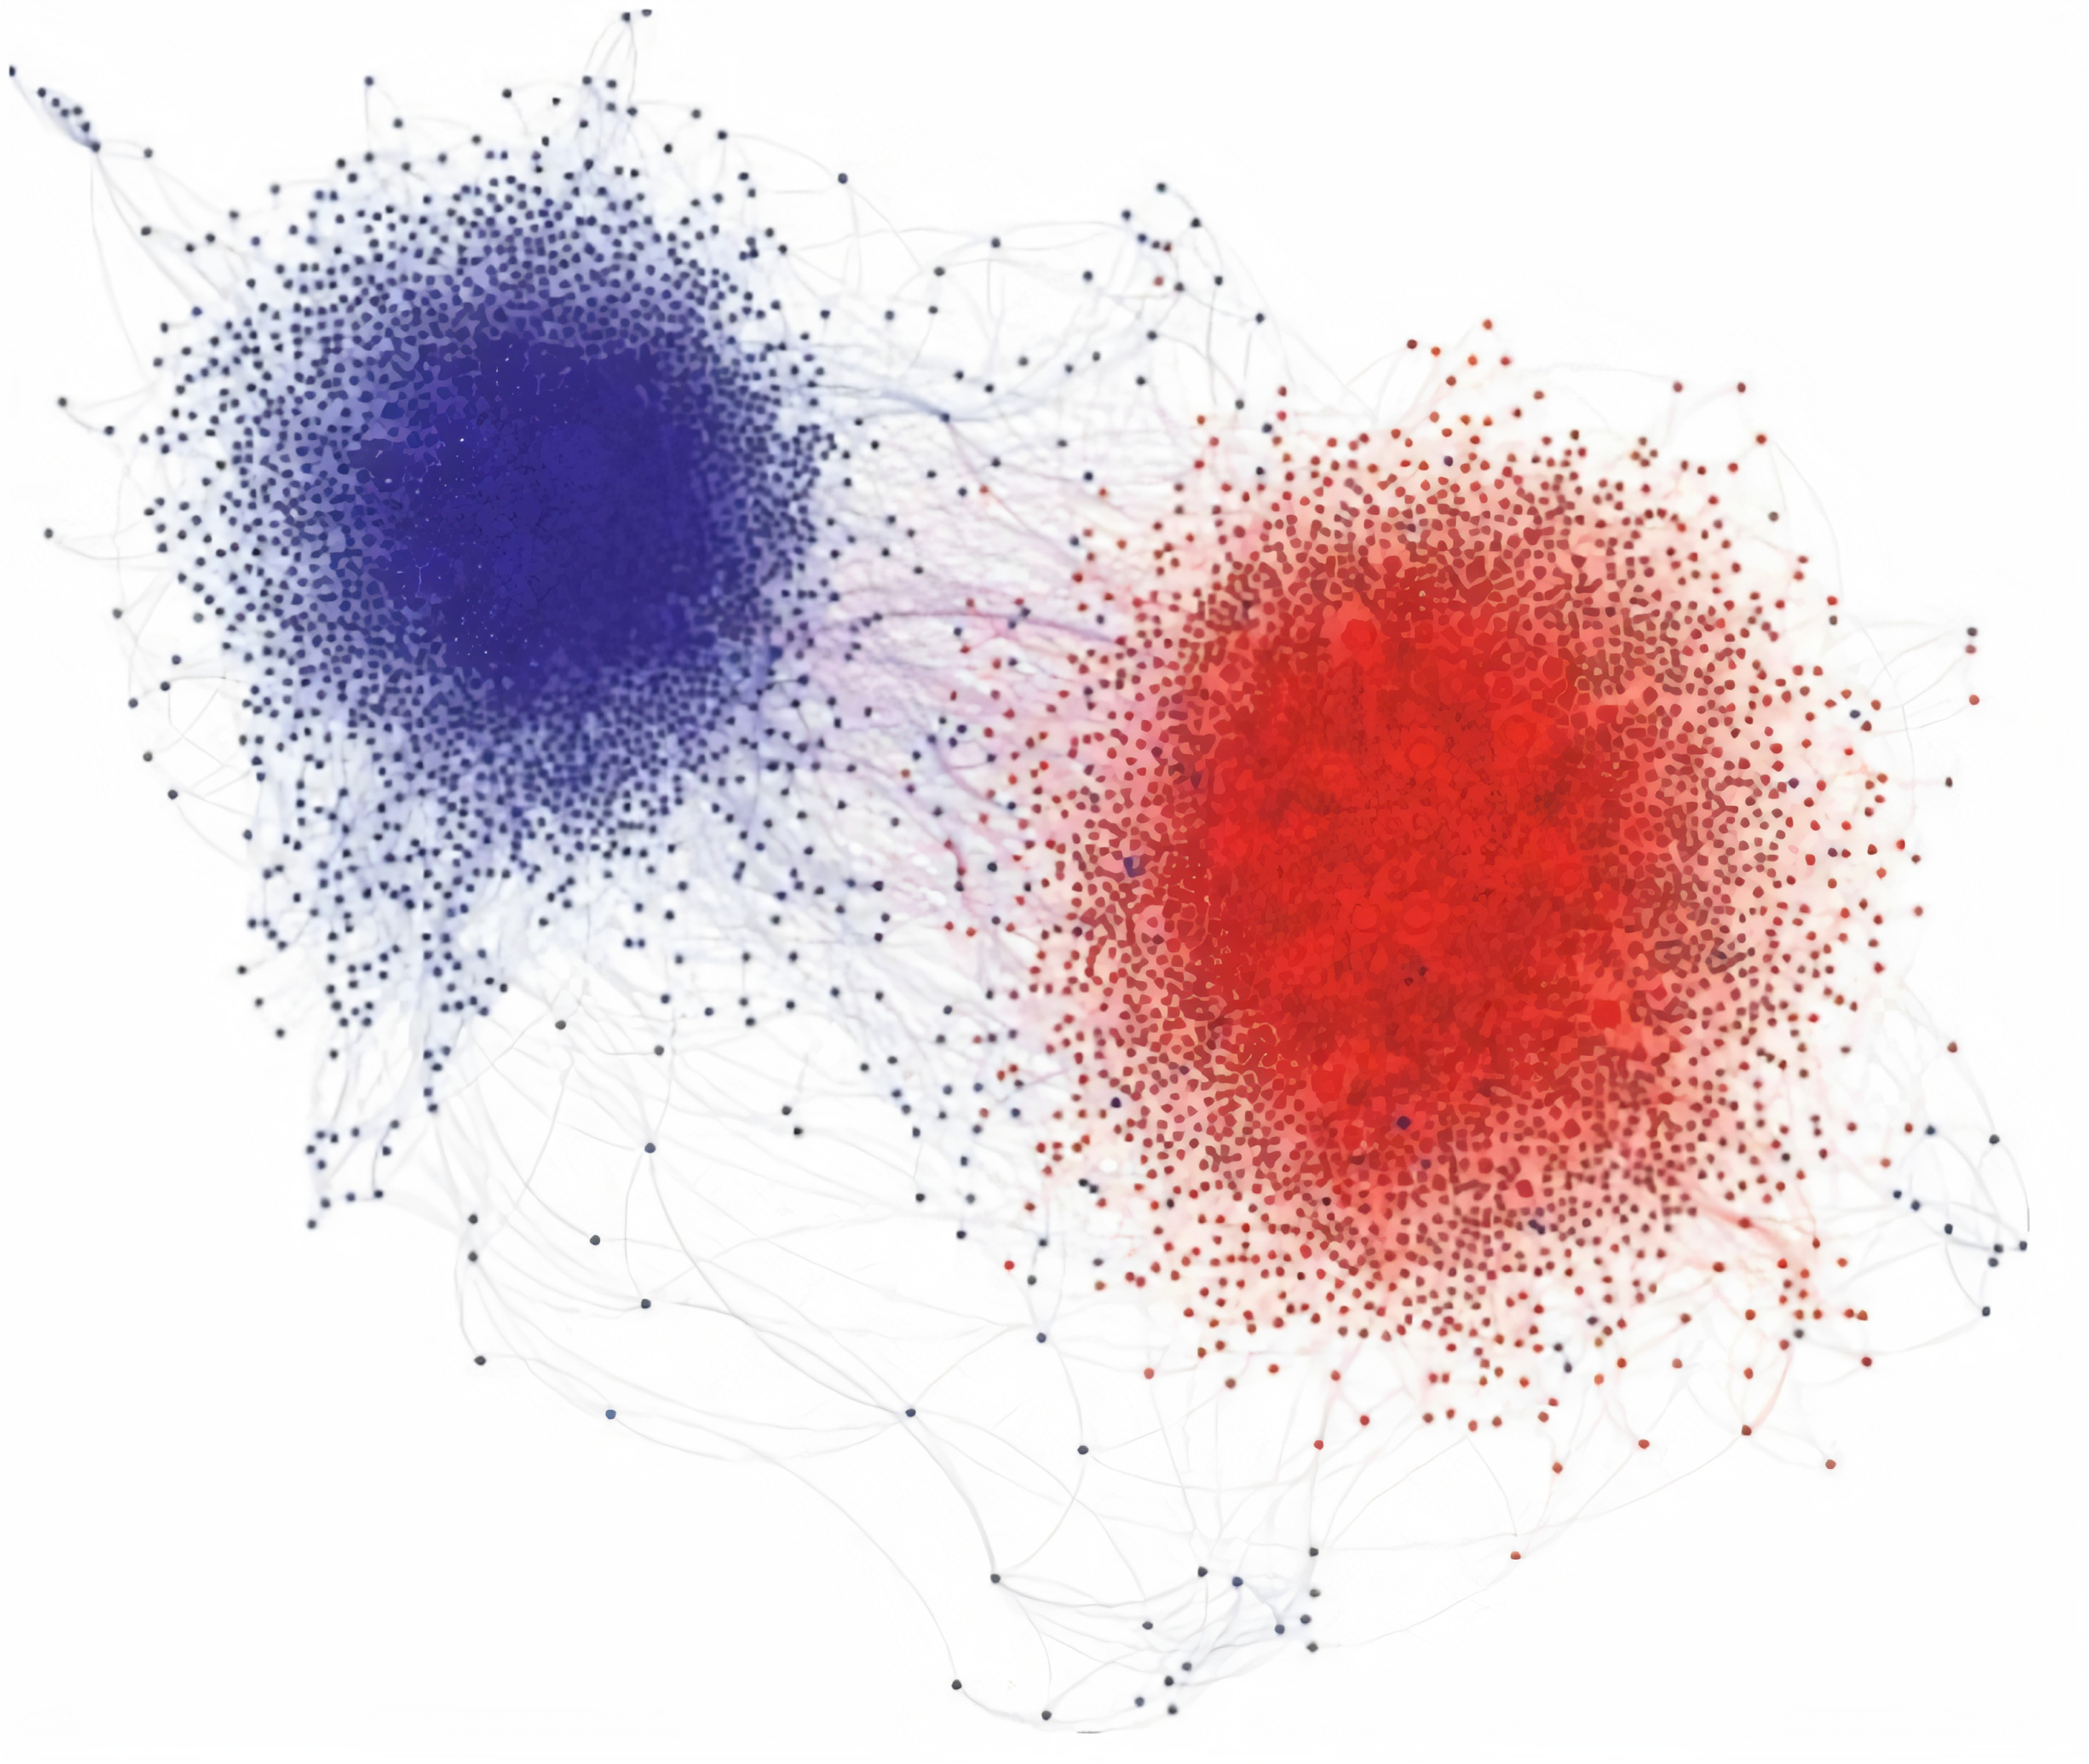
\includegraphics[width=0.6\linewidth]{tex/img/sample-graph.png}
	\caption[Retweet network during 2010 midterm elections]{The retweet network of posts regarding US during 2010 midterm
		elections. Red and blue nodes are associated with conservative and
		progressive users, respectively \cite{Menczer2020}}%
	\label{fig:tex/img/sample-graph}
\end{figure}

\paragraph{Different types of graphs}%
\label{par:different_types_of_graphs}

In its simplest form graph are \emph{undirected} and \emph{unweighted}. In an
\emph{undirected} graph relationships are bi-directional, while in directed graph
the order of nodes in a link reflects the
direction (i.e. an edge $e_{ij} $ is different from an edge $e_{ji} $). A weighted
graph instead associates a weight $\omega $ to each edge
\cite{Menczer2020}\cite{AlbertLaszloNortheasternUniversity2016}.

Sometimes also edges are allowed to be either positive or negative (for example when
definying the relationships in a acquaintance network): these king of networks
are usually called \emph{signed graphs} \cite{Newman2018}.

\bigskip

In the rest of the document we will abuse notation and refer to vertices both
as $v_{i} \in V $ and $i \in V$; similarly we will refer to edges both as
$e_{ij} \in E $ and as $ij \in E$.

\bigskip

Representing relationsips between entities which span over more than $2$
dimensions requires the definition of an ever more complex structure, the
\emph{multiplex graphs}, which is a collection of graphs (referred to as
\emph{layers}) over the same set of vertices, where each layer could represent
a different type of connection \cite{Newman2018}.

\section{Problem}
\label{sec:problem}

\subsection{The Interaction Graph}
\label{sub:interaction-graph}

The \emph{Interaction Graph} $G$ is the graph which encodes the informations
regarding the interactions between the users.

In this graph each users is associated to a vertex $v \in V$ and each edge to
an interaction between the $2$ corresponding users it links. For this reason we
will sometime refer to vertices as users in the rest of the document.

$G = (V, E^{+}, E^{-})  $ is a
signed and weighted graph, the weights being in the interval $[-1, +1]$,
corresponding to positive and negative interactions, meaning that for smaller
the value of the weight the interaction will more "negative".

The \emph{Interaction Graph} is also directed, so that an edge from vertex $v_{i}
$ to vertex $v_{j} $ corresponds to a reply from user $v_{i} $ to $v_{j} $.

Let a content $C$ be any kind of resource that triggers a discussion in one or
more threads $T$. The set of threads associated to $C$ is denoted as
$\mathcal{T}_{C} $. A content is usually represented by a newspaper article and
it is identified by its url, e.g.

	{\footnotesize
		\begin{center}
			\url{https://www.nytimes.com/2021/03/04/us/richard-barnett-pelosi-tantrum.html}
		\end{center}
	}

A corresponding thread may then be, for example, a user posting and commenting
the same url on its Twitter account (see \autoref{fig:twitter-thread}), thus
generating a discussion.

\begin{figure}
	\centering
	\includegraphics[width=0.6\linewidth]{tex/img/twitter_thread.png}
	\caption[Thread-content distinction example from Twitter]{An thread associated to the mentioned New York Times article}%
	\label{fig:twitter-thread}
\end{figure}

The \emph{Interaction Graph} is a \emph{multiplex graph}, each layer being
represented by a thread $T$ whose edges are the interactions happening in it.
Note also that for this reason each of the layers can contain more than one
edge between $2$ users, as each pair of users can reply to each other more than
once.

We will also use $\mathcal{C} $ for denoting the set of contents.

An example of \emph{Interaction Graph} can be seen in
\autoref{fig:interaction-graph-example}.

\begin{figure}
	\begin{center}
		\begin{subfigure}[b]{0.3\textwidth}
			\centering
			\tikzfig{tex/tikz/graph_thread1}
			\caption{$T_{1} \in \mathcal{T}_{C_{1}} $}
			\label{fig:tex/tikz/graph_thread1.tikz}
		\end{subfigure}
		\begin{subfigure}[b]{0.3\textwidth}
			\centering
			\tikzfig{tex/tikz/graph_thread2}
			\caption{$T_{2} \in \mathcal{T}_{C_{1}} $}
			\label{fig:tex/tikz/graph_thread2.tikz}
		\end{subfigure}
		\begin{subfigure}[b]{0.3\textwidth}
			\centering
			\tikzfig{tex/tikz/graph_thread3}
			\caption{$T_{3} \in \mathcal{T}_{C_{2}} $}
			\label{fig:tex/tikz/graph_thread3.tikz}
		\end{subfigure}
	\end{center}
	\caption[Example \emph{Interaction Graph}]{An example of \emph{Interaction Graph}, green and red edges
		representing positive and negative interactions, respectively. It
		contains $3$ threads and $2$ contents, the first $2$ layers each being
		associated to a thread of content $C_{1} $, the last layer to a thread
		of content $C_{2} $}
	\label{fig:interaction-graph-example}
\end{figure}

\subsection{The problem definition}%
\label{sub:the_problem_definition}

The main goal of the research is finding echo chambers in social medias, more
specifically on the \emph{Interaction Graph} as defined in
\autoref{sub:interaction-graph}.

Our definition is based on the idea that echo chambers can be identified by
looking at contents which is generally highly debated (we will call
this type of content \emph{controversial}) but which is discussed with little
or no animosity in small subgraphs. This subgraphs are the \emph{Echo
	Chambers}.

\bigskip

Given an \emph{Interaction Graph} $G = (V, E^{+}, E^{-})$ on some contents
$\mathcal{C} $ and threads, let $\eta(T)$ the number of negative edges over the
total number of edges in the layer associated to thread $T$. Similarly,
let $\eta(C)$ be the fraction of negative edges in all threads associated to
content $C$.

\begin{definition}[Controversial thread]
	Let $\alpha \in [0,1]$. A thread (or content) is \emph{controversial} if
	$\eta(T) > \alpha$ (or, similarly, $\eta(C) > \alpha $). Conversely, a
	thread (or content) is \emph{non-controversial} if $\eta(T) \leq \alpha$
	($\eta(C) \leq \alpha$).
\end{definition}

Intutively, \emph{controversial} threads contain many negative
interactions. We denote as $\hat{\mathcal{C} } \subseteq \mathcal{C} $ the
set of \emph{controversial} contents.

\medskip

\emph{Echo Chambers} correspond to \emph{non-controversial} smaller subgraphs
(i.e. with few negative edges) discussing a
\emph{controversial} content.

More formally, let $T[U]$ the subgraph induced in the layer associated to
thread $T$ by the vertices $U$; let $|T^{+} [U]|$ and $|T^{-} [U]|$ its number
of positive and negative edges, respectively.

We define $\mathcal{S}_C (U)$ as the set of \emph{non-controversial} threads
induced by $U$, for \textit{controversial} contents, i.e.
	{\small
		\begin{equation}
			\mathcal{S} _{C} (U) = \{ T[U] \; s.t. \; T[U] \; non \;
			controversial, T \in \mathcal{T} _{C}, C
			\in \hat{\mathcal{C}}, U \subseteq V\}
		\end{equation}
	}

Thus $\mathcal{S} _C (U)$ will contain threads which are \emph{globally} non
controversial but it is defined only for contents that are \emph{globally}
controversial.

\medskip

We know define the Echo Chamber Score of a set of vertices $U$.

\begin{definition}[Echo Chamber Score]
	Let $U \subseteq V$ be a subset of vertices. Its Echo Chamber Score is

	\begin{equation}
		\label{eq:echo-chamber-score}
		\xi(U) = \sum^{}_{\mathcal{C} \in \mathcal{\hat{C}}} \sum^{}_{T[U] \in
		\mathcal{S} _{C} (U)} (|T^{+} [U]| - |T ^{-} [U]|)
	\end{equation}
\end{definition}

We can now define the \acrfull{ECP}.

\begin{problem}[\acrfull{ECP}]
Given an \emph{Interaction Graph} $G$ and $\alpha \in [0, 1]$ find a set of vertices $U \subseteq
	V$ maximizing the Echo Chamber Score (\autoref{eq:echo-chamber-score}).
\end{problem}

We will denote with $\hat{U}$ the set of users maximizing
\autoref{eq:echo-chamber-score} and with $\xi(G)$ its corresponding score, i.e.

\begin{align*}
	\hat{U} & \coloneqq \argmax_{U \subseteq V} \xi(U) & \xi(G) & \coloneqq
	\xi(\hat{U})
\end{align*}

\subsection{The Densest Echo Chamber Problem}%
\label{sub:the_densest_echo_chamber_problem}

The \acrshort{ECP} doesn't take into account the number of users producing a
certain score; this means that the set $U$ may involve disconnected and sparse
subgraphs, depending on the structure of the graph $G$.

For this reason it is interesting also to study another variant of the
\acrshort{ECP}, the \acrlong{D-ECP}, which we now define.

\begin{definition}[Echo Chamber Score]
	Let $U \subseteq V$ be a subset of vertices. Its Densest Echo Chamber Score is

	\begin{equation}
		\label{eq:densest-echo-chamber-score}
		\xi(U) = \sum^{}_{\mathcal{C} \in \mathcal{\hat{C}}} \sum^{}_{T[U] \in
		\mathcal{S} _{C} (U)} \frac{(|T^{+} [U]| - |T ^{-} [U]|)}{|U|}
	\end{equation}
\end{definition}

Similarly to the \acrshort{ECP} we can now define the corresponding problem

\begin{problem}[\acrfull{D-ECP}]
Given an \emph{Interaction Graph} $G$ and $\alpha \in [0, 1]$ find a set of vertices $U \subseteq
	V$ maximizing the Densest Echo Chamber Score (\autoref{eq:densest-echo-chamber-score}).
\end{problem}

\section{Goals}
\label{sec:goals}

In this document we address the following research questions:

\begin{enumerate}
	\item Can we solve the \acrlong{ECP} and the \acrlong{D-ECP}?
	\item Are the \acrlong{ECP} and the \acrlong{D-ECP} capable of finding echo
	      chambers inside social medias?
\end{enumerate}

\section{Structure of the thesis}
\label{sec:structure-thesis}

% todo

\section{About the thesis}
\label{sec:about-thesis}

The code which was used to obtain the results presented in the rest of the
document is available at the following GitHub address

\begin{center}
	\url{https://github.com/morpheusthewhite/master-thesis}
\end{center}

% \cleardoublepage
% \chapter{Background}
\label{ch:background}

This chapter provides the background knowledge relevant for the thesis work. It
will initially discuss graph and related problems (\autoref{sec:signed_graphs_and_density}) which are significant in the
following used methodologies, as well as concepts of computational complexity
(\autoref{sec:computational_complexity_and_approximability}) and Linear
Programming (\autoref{sec:linear_and_mixed_integer_programming}).

\section{Signed graphs and density}%
\label{sec:signed_graphs_and_density}

\section{Computational complexity and \\approximability}%
\label{sec:computational_complexity_and_approximability}

Complexity Theory deals with the study of the intrinsic complexity of
computational tasks; more specifically it mainly aims at determining the
complexity of any given task. It also elaborates on the relationships between
the complexity of different problems, for example proving that 2 problems are
computationally equivalent\cite{9780521884730}, through a notion called
\emph{reduction}.

\subsection{Complexity classes}%
\label{par:complexity_classes}

According to their complexity, problems can be divided in different groups
\cite{DemaineFall2014}.

\paragraph{$\mathcal{P} $}%
\label{par:p}
is the set of problems which can be solved in polynomial time in the size $n$ of
the problem, i.e. $n^{O(1)} $. In this set there are problems such as Linear
Programming Models \cite{KHACHIYAN198053}\cite{Karmarkar1984}, finding whether
or not a graph is connected \cite{9780521884730}.

\paragraph{$\mathcal{NP} $}%
\label{par:np} is the set of problems whose solution can be verified in
polynomial time in the size $n$ of the problem, i.e. $n^{O(1)} $.

According to these definition it is easy to see that $\mathcal{P} \subseteq
	\mathcal{NP} $. A common $\mathcal{NP} $ problem is factoring, i.e. finding a
prime factor $p$ of a number $N$ in a given interval \cite{SanjeevArora2017}.

\paragraph{$\mathcal{NP} $-Hard}%
\label{par:_np_hard} is the set of problems that are \emph{at least as hard} as
any other problem in $\mathcal{NP} $. Some well-known $\mathcal{NP} $-Hard
problems are the $\textsc{Sat}$ (deciding whether a boolean formula can be
satisfied or not) and the $\textsc{MaxClique}$ (finding the biggest complete
subgraph), as shown is a famous paper by Karp \cite{Miller1972} (see
\autoref{fig:tex/img/post_vaccine_social_scheduling} ).

\begin{figure}[]
	\centering
	\includegraphics[width=0.8\linewidth]{tex/img/post_vaccine_social_scheduling.png}
	\caption{\emph{As if this problems weren't $\mathcal{NP} $-Hard enough}.
		Post-vaccine social scheduling may be $\mathcal{NP} $-Hard \cite{Munroe}}%
	\label{fig:tex/img/post_vaccine_social_scheduling}
\end{figure}

\paragraph{$\mathcal{NP} $-Complete}%
\label{par:_np_hard} is the set of problems in $\mathcal{NP} $-Hard that are
also in $\mathcal{NP} $. Intuitively these correspond the most difficult
problems to solve in $\mathcal{NP} $. The number of problems which are known to
be in this set is in the order of a thousand \cite{SanjeevArora2017}.

\subsection{$\mathcal{P} $ vs $\mathcal{NP}$}%
\label{sub:_p_vs_np_}

A fundamental question in Computational Complexity is wheter $\mathcal{P} =
	\mathcal{NP} $. Mostly people believe that this is not true, so
$\mathcal{P} \neq \mathcal{NP} $, and also our daily experience tell us that
often it is easier to check the correctness of a solution of a problem than
finding it \cite{9780521884730}: in many cases coming up with the correct
answer requires searching over an exponentially large set
\cite{SanjeevArora2017}. Nonetheless no mathematical proof of this notion has
been found and, in fact, in the last decades there has been little or no progress towards it \cite{Erickson2019}.

If, it is mostly accepted, $\mathcal{P} \neq \mathcal{NP} $ this would produce
a situation as depicted in \autoref{fig:tex/img/complexity-diagram}:
there are problems for which we are not able to find the solution
efficiently (i.e. in polynomial time). On the other side this allows the
existance of one-way-functions (i.e. functions whose inverse is much harder to
compute than the original functions) on which Modern Criptography heavily
relies \cite{9780521884730}.
%
% This brings the need for algorithms which are able to approximate the solution
% in a reasonable amount of time.

% Viceversa, if $\mathcal{P} = \mathcal{NP} $, it would be very easy to find
% proofs and mathematicians could be replaced by
% look at 2.7.3 in Sanjeev's book

\begin{figure}
	\centering
	\includegraphics[width=0.3\linewidth]{tex/img/complexity-diagram.png}
	\caption{Venn diagram for the complexity classes if $\mathcal{P} \neq
			\mathcal{NP} $ \cite{article}}%
	\label{fig:tex/img/complexity-diagram}
\end{figure}

\subsection{Optimization Problems and $\mathcal{NPO} $}%
\label{sub:optimization_problems}

Optimization problems are defined from a problem instance $x$, a set of
feasible solutions $S$ and a cost function that takes as input the problem
instance $x$ a feasible solution $s \in S$, denoted as cost$_{O} (x, s) $.
Given a minimization (maximization) problem the optimal solution is defined as
the $s$ minimizing (maximizing) the value of cost$_{O} (x, s)$, and we denote
by opt$_{O} (x) $ this value\cite{Trevisan2004}.

\paragraph{$\mathcal{NPO} $}%
\label{par:_npo_}

is then the set of optimization problems whose cost function
can be computed in polynomial time and for every instance of the problem $x$
and feasible solution for that problem $s \in A$ there is a polynomial $q \; s.t.
	\; s \leq q(|x|)$ (i.e. the size of every solution is bounded by a polynomial
in $x$).

If $\mathcal{P} \neq \mathcal{NP} $ for many optimization problems there is no
algorithm for finding the optimal solution in polynomial time
\cite{Trevisan2004}. This is again a fundamental limitation about what we can
compute which then requires the definition of some alternative approaches, like
the definition of \emph{approximation algorithm}
which are able to be computed in polynomial time
a solution which lies in a given factor from the optimal
one\cite{Vazirani2002}.

\paragraph{Approximation}%
\label{par:r_approximations}

$A$ is an r-approximation algorithm for an $\mathcal{NPO} $ minimization
problem $O$ if, for every instance $x$ of $O$ it holds that
\begin{equation*}
	cost_{O} (x, A(x)) \leq r \cdot opt_{O} (x)
\end{equation*}

\noindent
(or, respectively, cost$_{O} (x, A(x))
	\leq 1/r \cdot $opt$_{O} (x) $ for maximization problems), $A(x)$ being the
optimal solution found by the approximation algorithm \cite{Trevisan2004}.

\subsection{Approximation preserving reductions}%
\label{sub:approximation_preserving_reductions}

Problems approximability varies widely: while for some of them exists
constant factor approximations, for some others even a remotely approximate
solution cannot be found \cite{Ausiello2005} (some examples are listed in
\autoref{tab:inapproximability-examples} ).

% todo: reference to the papers proving each result instead of the hub
\begin{table}
	\centering
	\caption{Examples of known inapproximability results, assuming $\mathcal{P}
			\neq \mathcal{NP} $ \cite{10.1007/3-540-63248-4_10} }
	\label{tab:inapproximability-examples}
	\begin{tabular}{c|p{5cm}|c}
		Problem                                                          & Description                                                   & Inapproximability \\
		\hline
		$ \textsc{MaxClique} $                                           & Biggest complete subgraph                                     & $|V|^{1-
		\epsilon}, \forall \epsilon > 0 $                                                                                                                    \\
		                                                                 &                                                               &                   \\
		$ \textsc{MaximumIndipendentSet} $                               &
		Biggest set of not connected nodes                               & $|V|^{1-
		\epsilon}, \forall \epsilon > 0 $                                                                                                                    \\
		                                                                 &                                                               &                   \\
		$ \textsc{MinCut} $                                              & Partition of nodes in 2 sets $V_1$ and $V_2$ minimizing edges
		between the 2 sets                                               & 1.0624                                                                            \\
		                                                                 &                                                               &                   \\
		$ \textsc{MaximumSetPacking} $                                   & Given a collection of
		finite sets $C$,
		finding the biggest collection $C' \subseteq C$ of disjoint sets & $|C|^{1-
		\epsilon}, \forall \epsilon > 0 $                                                                                                                    \\
	\end{tabular}
\end{table}

\emph{Approximation preserving reductions} are a fundamental notion for proving
a partial order among optimization problems \cite{Ausiello2005}. An
\emph{Approximation preserving reductions} must have
the following properties (when reducing from a problem $A$ to a problem $B$)
\cite{DemaineFall2014}:

\begin{itemize}
	\item any instance $x$ of $A$ should be mapped to an instance $x' = f(x)$
	      of $B$ in polynomial time
	\item any solution $y' \in $ sol$(f(x))$ of $B$ should be associated to a corresponding
	      solution $y = g(x, y') \in $ sol$(x)$ of $A$ in polynomial time
\end{itemize}

So there are 2 efficient (i.e. requiring polynomial time) functions $f$ and $g$
for mapping instances of $A$ to $B$ and solution of $B$ to solutions of $A$,
respectively (\autoref{fig:tex/img/reduction_scheme}).

\begin{figure}
	\centering
	\includegraphics[width=0.6\linewidth]{tex/img/reduction_scheme.png}
	\caption{The reduction scheme \cite{Crescenzi1997ASG}}%
	\label{fig:tex/img/reduction_scheme}
\end{figure}

There are at least 9 different kinds of approximation preserving reductions
\cite{DemaineFall2014}(\autoref{fig:tex/img/approximation_preserving_reductions}) but we will
focus only on one type.

\begin{figure}[b]
	\centering
	\includegraphics[width=0.4\linewidth]{tex/img/approximation_preserving_reductions.png}
	\caption{Taxonomy of approximation preserving reductions \cite{Crescenzi1997ASG}}%
	\label{fig:tex/img/approximation_preserving_reductions}
\end{figure}

\subsubsection{S reductions}%
\label{sub:strict_reductions}

An $S$ \emph{reduction} from problem $A$ to problem $B$ has the following properties \cite{Crescenzi1997ASG}:
\begin{itemize}
	\item fox any instance $x$ of problem $A$ it holds that opt$_{A} (x) = $ opt$_{B} (f(x))$
	\item for any instance $x$ of $A$ and solution $y'$ of $B$, cost$_{A} (x,
		      g(x, y')) = $ cost$_{B} (f(x), y')$
\end{itemize}

Strict reductions are the strongest type of \emph{approximation preserving
	reductions} and imply all the others \cite{Crescenzi1997ASG}.

\clearpage

\section{Linear and Mixed Integer Programming}%
\label{sec:linear_and_mixed_integer_programming}

\acrlong{LP} is a widely used optimization technique and one of the most
effective; the term refers to problems in which both the constraints and \emph{objective
	function} are linear
\cite{Edgar2001}\cite{Vanderbei2008}\cite{Dantzig1998}\cite{Martin1998}.

\subsection{The structure of a linear programming model}%
\label{sub:the_structure_of_a_linear_programming_model}

In a \acrfull{LP} problem we are given a cost vector $ \mathbf{c} = (c_1,
	\dots, c_n) $ and we want to minimize (or maximize) a linear cost function over
the variables $ \mathbf{x} = (x_1, \dots, x_n) $ with the coefficients of the
cost vector $ \mathbf{c} $, i.e.
\begin{equation*}
	\mathbf{cx} = \sum^{n}_{i=1} c_i x_i
\end{equation*}
(known as the \emph{objective function}) while satisfying some linear
constraints over the variables \cite{Bertsimas1997}\cite{Vanderbei2008}:

\begin{equation*}
	a_1 x_1 + \dots + a_n x_n \begin{Bmatrix} \leq \\ = \\ \geq \end{Bmatrix} b
\end{equation*}

% There is no \emp{a priori} preference regarding how the problem is formulated
% since it is easy to convert an inequality into a equality constraint through
% additional variables ($\omega $ in the example below) called \emph{slack}
% \cite{Vanderbei2008}. For example one in the form
% \begin{equation*}
%     a_1 x_1 + \dots + a_n x_n \leq b
% \end{equation*}
% is equivalent to
% \begin{equation*}
%     a_1 x_1 + \dots + a_n x_n + \omega = b, \quad \omega \geq 0
% \end{equation*}
% and viceversa an equality
% \begin{equation*}
%     a_1 x_1 + \dots + a_n x_n = b
% \end{equation*}
% can be converted into
% \begin{align*}
%     a_1 x_1 + \dots + a_n x_n \leq b \\
%     a_1 x_1 + \dots + a_n x_n \geq b
% \end{align*}
%
In general is possible to formulate any \acrshort{LP} problem as follows (called \emph{standard form}) \cite{Vanderbei2008}

\begin{alignat*}{2}
	 & \text{minimize}   &       & \sum_{i=1}^{m} c_{i}x_{i} \\
	 & \text{subiect to} & \quad &
	\begin{aligned}[t]
		\sum_{i=1}^{n} a_{1i}  x_{i} & \leq b_{1} &                        \\
		\vdots                                                             \\
		\sum_{i=1}^{n} a_{mi}  x_{i} & \leq b_{m} &                        \\
		x_{i}                        & \geq 0,    & \quad i & =1 ,\dots, n
	\end{aligned}
\end{alignat*}

The $x_i$ are known also as \emph{decision variables}; a choice of $ \mathbf{x}
$ if called \emph{solution} and \emph{feasible solution} if it satisfies the
constraints, \emph{optimum} if it maximizes the \emph{objective function}
\cite{Vanderbei2008}.

\subsection{Solving an LP problem}%
\label{sub:solving_an_lp_problem}

\subsection{Mixed Integer Programming}%
\label{sub:mixed_integer_programming}

% \cleardoublepage
% \chapter{Methods}
\label{ch:methods}

This chapter focuses on describing the main topic of the
research: the problems are motivated and defined in
\autoref{sec:the_echo_chamber_problem}, and their complexity is then analyzed
in \autoref{sec:problem_complexity_and_approximability}, while proposing some
alternative problem definitions. Algorithms and models for solving and
approximating the problems are then proposed in
\autoref{sec:solving_the_problem}; the definition of a generative model
concludes the chapter (\autoref{sec:generative_model}).

\section{The \acrlong{ECP}}%
\label{sec:the_echo_chamber_problem}

This section starts by outlining the graph on which the analysis is carried
out (\autoref{sub:interaction-graph}), the process for building it
(\autoref{sub:collection_and_preprocessing}) and finally defines the
\acrlong{ECP} and the \acrlong{D-ECP} (\autoref{sub:the_problem_definition} and
\autoref{sub:the_densest_echo_chamber_problem}).

\subsection{The Interaction Graph}
\label{sub:interaction-graph}

The \emph{Interaction Graph} $G$ is the graph which encodes the informations
regarding the interactions between the users.

In this graph each users is associated to a vertex $v \in V$ and each edge to
an interaction between the $2$ corresponding users it links. For this reason we
will sometime refer to vertices as users in the rest of the document.

$G = (V, E^{+}, E^{-})  $ is a
signed and weighted graph, the weights being in the interval $[-1, +1]$,
corresponding to positive and negative interactions, meaning that for smaller
the value of the weight the interaction will more "negative".

The \emph{Interaction Graph} is also directed, so that an edge from vertex $v_{i}
$ to vertex $v_{j} $ corresponds to a reply from user $v_{i} $ to $v_{j} $.

Let a content $C$ be any kind of resource that triggers a discussion in one or
more threads $T$. The set of threads associated to $C$ is denoted as
$\mathcal{T}_{C} $. A content is usually represented by a newspaper article and
it is identified by its url, e.g.

	{\footnotesize
		\begin{center}
			\url{https://www.nytimes.com/2021/03/04/us/richard-barnett-pelosi-tantrum.html}
		\end{center}
	}

A corresponding thread may then be, for example, a user posting and commenting
the same url on its Twitter account (see \autoref{fig:twitter-thread}), thus
generating a discussion.

\begin{figure}
	\centering
	\includegraphics[width=0.6\linewidth]{tex/img/twitter_thread.png}
	\caption{An thread associated to the mentioned New York Times article}%
	\label{fig:twitter-thread}
\end{figure}

The \emph{Interaction Graph} is a \emph{multiplex graph}, each layer being
represented by a thread $T$ whose edges are the interactions happening in it.
Note also that for this reason each of the layers can contain more than one
edge between $2$ users, as each pair of users can reply to each other more than
once.

We will also use $\mathcal{C} $ for denoting the set of contents We will assume that $G = \bigcup _{C \in \mathcal{} } $

An example of \emph{Interaction Graph} can be seen in
\autoref{fig:interaction-graph-example}.

\begin{figure}
	\begin{center}
		\begin{subfigure}[b]{0.3\textwidth}
			\centering
			\tikzfig{tex/tikz/graph_thread1}
			\caption{$T_{1} \in \mathcal{T}_{C_{1}} $}
			\label{fig:tex/tikz/graph_thread1.tikz}
		\end{subfigure}
		\begin{subfigure}[b]{0.3\textwidth}
			\centering
			\tikzfig{tex/tikz/graph_thread2}
			\caption{$T_{2} \in \mathcal{T}_{C_{1}} $}
			\label{fig:tex/tikz/graph_thread2.tikz}
		\end{subfigure}
		\begin{subfigure}[b]{0.3\textwidth}
			\centering
			\tikzfig{tex/tikz/graph_thread3}
			\caption{$T_{3} \in \mathcal{T}_{C_{2}} $}
			\label{fig:tex/tikz/graph_thread3.tikz}
		\end{subfigure}
	\end{center}
	\caption{An example of \emph{Interaction Graph}, green and red edges
		representing positive and negative interactions, respectively. It
		contains $3$ threads and $2$ contents, the first $2$ layers each being
		associated to a thread of content $C_{1} $, the last layer to a thread
		of content $C_{2} $}
	\label{fig:interaction-graph-example}
\end{figure}

\subsection{Collection and preprocessing}%
\label{sub:collection_and_preprocessing}

% todo: data collection process and compliance with current legislation

\subsection{The problem definition}%
\label{sub:the_problem_definition}

\subsection{The Densest Echo Chamber Problem}%
\label{sub:the_densest_echo_chamber_problem}

\section{Problems complexity and approximability}%
\label{sec:problem_complexity_and_approximability}

\subsection{Hardness of ECP}%
\label{sub:ecp_is_}

\subsection{Hardness of D-ECP}%
\label{sub:ecp_is_}

\subsection{Solvable variants of the problem}%
\label{sub:solvable_variants_of_the_problem}

\section{Solving the problem}%
\label{sec:solving_the_problem}

\subsection{A MIP model for the ECP}%
\label{sub:a_mip_model_for_the_ecp}

\subsection{A MIP model for the D-ECP}%
\label{sub:a_mip_model_for_the_ecp}

\subsection{Approximation algorithms}%
\label{sub:approximation_algorithms}

\section{A generative model}%
\label{sec:generative_model}



% \subsection{Validity of method}
% \todo[inline]{How will you know if your results are valid?}

% \cleardoublepage
% \chapter{What you did}\todo[inline]{Choose your own chapter title to describe this}
\todo[inline, backgroundcolor=aqua]{[Vad gjorde du? Hur gick det till? – Välj lämplig rubrik (“Genomförande”, “Konstruktion”, ”Utveckling”  eller annat]}
\label{ch:whatYouDid}

\todo[inline]{What have you done? How did you do it? What design decisions did you make? How did what you did help you to meet your goals?}
\begin{swedishnotes}
	Vad du har gjort? Hur gjorde du det? Vad designen beslut gjorde du?
	Hur kom det du hjälpte dig att uppnå dina mål?
\end{swedishnotes}

\section{Hardware/Software design …/Model/Simulation model \& parameters/…}
\todo[inline, backgroundcolor=aqua]{Hårdvara / Mjukvarudesign ... / modell / Simuleringsmodell och parametrar / …}

Figure~\ref{fig:homepageicon} shows a simple icon for a home page. The time
to access this page when served will be quantified in a series of
experiments. The configurations that have been tested in the test bed are
listed in Table~\ref{tab:configstested}.

\begin{swedishnotes}
	Figur~\ref{fig:homepageicon}  visar en enkel ikon för en hemsida. Tiden för att få tillgång till den här sidan när serveras kommer att kvantifieras i en serie experiment. De konfigurationer som har testats i provbänk listas ini tabell~\ref{tab:configstested}.

	Vad du har gjort? Hur gjorde du det? Vad designen beslut gjorde du?
\end{swedishnotes}

\begin{table}[!ht]
	\begin{center}
		\caption{Configurations tested}
		\label{tab:configstested}
		\begin{tabular}{l|c} % <-- Alignments: 1st column left, 2nd middle and 3rd right, with vertical lines in between
			\textbf{Configuration} & \textbf{Description}        \\
			\hline
			1                      & Simple test with one server \\
			2                      & Simple test with one server \\
		\end{tabular}
	\end{center}
\end{table}
\todo[inline, backgroundcolor=aqua]{Konfigurationer testade}

\section{Implementation …/Modeling/Simulation/…}
\todo[inline, backgroundcolor=aqua]{Implementering … / modellering / simulering / …}
\label{sec:implementationDetails}

\subsection{Some examples of coding}

Listing~\ref{lst:helloWorldInC} shows an example of a simple program written
in C code.

\begin{lstlisting}[language={C}, caption={Hello world in C code}, label=lst:helloWorldInC]
int main() {
printf("hello, world");
return 0;
}
\end{lstlisting}


In contrast, Listing~\ref{lst:programmes} is an example of code in Python to
get a list of all of the programs at KTH.

\lstset{extendedchars=true}
\begin{lstlisting}[language={Python}, caption={Using a python program to
    access the KTH API to get all of the programs at KTH}, label=lst:programmes]
KOPPSbaseUrl = 'https://www.kth.se'

def v1_get_programmes():
    global Verbose_Flag
    #
    # Use the KOPPS API to get the data
    # note that this returns XML
    url = "{0}/api/kopps/v1/programme".format(KOPPSbaseUrl)
    if Verbose_Flag:
        print("url: " + url)
    #
    r = requests.get(url)
    if Verbose_Flag:
        print("result of getting v1 programme: {}".format(r.text))
    #
    if r.status_code == requests.codes.ok:
        return r.text           # simply return the XML
    #
    return None
\end{lstlisting}


% \cleardoublepage
%
% \chapter{Results and Analysis}
\label{ch:resultsAndAnalysis}

\section{Data collection and generation}%
\label{sec:data_collection_and_generation}

We now discuss how the real-world data is retrieved and preprocessed as well as
presenting some techniques for generatic synthetic data.

\subsection{Collection and preprocessing}%
\label{sub:collection_and_preprocessing}

Datasets are built mainly upon $2$ social medias: Twitter and Reddit; the data
collection process, consequently, slightly differ between them.

\paragraph{Twitter}%
\label{par:twitter-data}

Twitter's \emph{Interaction Graphs} are mainly built starting from the tweets
of some important social accounts associated to well-known news source, like The
New York Times or Fox News, that tipically post links to their articles:
these profiles are taken as the source of the contents $\mathcal{C} $ of the graph.

Each time another user tweets the same url (\autoref{fig:twitter-thread}) then
it will correspond to another thread related to the same content, and all the
replies it receives will be part of this new thread.

Twitter data is retrieved with the help of Tweepy \cite{tweepy}, a Python
library for accessing the Twitter API, which has been patched for using some
features available only in the beta of the new Twitter API (v2).

\paragraph{Reddit}%
\label{par:reddit}

Differently from Twitter, Reddit focuses on subreddits, which are pages
collecting posts from different users about a specific topic (e.g. r/politics,
r/economics, $\dots$). This means that
in the datasets built from this social media the contents $\mathcal{C} $ is the
set of posts of these pages, which, differently from Twitter, most likely
come from different sources.

This posts are in turn crossposted, i.e. reposted on other subreddits. Each of
these \emph{crosspost} will eventually correspond to another thread.

The PRAW library is used for retrieving the data \cite{praw}.

\paragraph{Edge weights assignment}%
\label{par:assigning_edge_weights}

Once the threads interactions are retrieved they are passed to a state of the
art sentiment analyzer which labels them. More specifically the model used is
RoBERTa which has been adapted and retrained for dealing with Twitter
data \cite{Barbieri2020}. The model is made available by the Transformers
python library \cite{wolf-etal-2020-transformers}.

\bigskip

Finally, complying with the current privacy legislation, all the data related
to the user is pseudo-anonymized (accounts identifier are replaced by random
ones) while no data is publicly available.

\subsection{Synthetic data}%
\label{sub:synthetic_data}

Here we propose $2$ possible methods for generating data, the Signed SBM and
the Information spread Model.

\subsubsection{Signed SBM}%
\label{ssub:signed_sbm}

This model is very similar to the Stochastic Block Model (SBM), a model
commonly used for generating random graphs having some community structures
\cite{Newman2018}.

The Signed SBM is based on the following parameters
\begin{itemize}
	\item $b_{i} $, the group assignment of each vertex $i$
	\item $\omega ^{+} _{rs} $ and $\omega ^{-} _{rs} $, the probabilities
	      of positive and negative edges, respectively, between users in
	      group $r$ and $s$. Vertices have also a probability of not having an
	      edge, which is equal to $1 - \omega ^{-} _{rs} - \omega ^{+} _{rs} $.
	      For this reason it is clearly needed that $\omega ^{+} _{rs} + \omega ^{-} _{rs} \leq 1$.
	\item $\theta \leq 1$, controlling the reduction of probability of interacting
	      between \emph{inactive} communities
\end{itemize}

Therefore, generating a thread layer\footnote{in this model we will generate contents univocally associated to threads} for the \emph{Interaction Graph} involves the following process
\begin{enumerate}
	\item Sample $n'$ among the $n$ communities. These are the
	      \emph{active} communities in the discussion of the thread
	\item For each node pairing $i, j$ consider their corresponding groups $r$ and
	      $s$ and draw from one of the following categorical distribution to decide to add
	      a positive, negative or no edge.
	      \begin{itemize}
		      \item If both communities $r$ and $s$ are \emph{active}
		            \begin{equation*}
			            (\omega _{rs} ^{+}, \omega _{rs} ^{-}, 1 - \omega _{rs} ^{+} - \omega _{rs} ^{-})
		            \end{equation*}
		      \item otherwise
		            \begin{equation*}
			            (\theta \omega _{rs} ^{+}, \theta \omega _{rs} ^{-}, 1 - \theta (\omega _{rs} ^{+} + \omega _{rs} ^{-}))
		            \end{equation*}

	      \end{itemize}

\end{enumerate}

\subsubsection{Information spread model}%
\label{ssub:information_spread_model}

Here we describe the Information spread model, which aims at simulating the
process of informations flowing between different users of a social media.

Like in the Signed SBM, each node has a group assignment and there are probabilities of
positive and negative edges $\omega _{rs}^{+}  $ and $\omega _{rs}^{+}  $,
respectively, with $\omega ^{-} _{rs} + \omega ^{+} _{rs}
	\leq 1$. Additionally, we have the following new parameters

\begin{itemize}
	\item ${\phi_{rs} }$, the parameters of a standard SBM
	\item $\beta _a$, the probability that a node is initially activated
	\item $\beta _n$, the probability the an inactive node is activated
	      from a friend
\end{itemize}

\bigskip
Generate the \emph{follow} graph $G_{f}$ from a SBM with parameters $\{ \phi
	_{rs}  \}$; we will refer to neighbours in this graph as \emph{friends}.
The generation of a thread for the \emph{Interaction Graph} goes as follows

\begin{enumerate}
	\item Activate vertices with probability $\beta_{a}  $
	\item Any of these active nodes activates its inactive friends with
	      probability $\beta_n$
	      % \item Let $a_{i} $ be the number of \emph{active} neighbours of node
	      %     $i$ in $G$ and $m_{i} $ the number of neighbours of node $i$ in
	      %     $G$. Any node inactive from the previous step is activated with
	      %     probability $ \frac{a_i}{m_i} \beta _{n} $
	\item Similarly to before, if $2$ nodes are both active nodes they will interact according to the categorical distribution
	      \begin{equation*}
		      (\omega _{rs}
		      ^{+}, \omega _{rs} ^{-}, 1 - \omega _{rs} ^{+} - \omega _{rs} ^{-})
	      \end{equation*}

	      otherwise according to
	      \begin{equation*}
		      (\theta \omega _{rs} ^{+}, \theta \omega _{rs} ^{-}, 1
		      - \theta (\omega _{rs} ^{+} + \omega _{rs} ^{-}))
	      \end{equation*}
\end{enumerate}

\section{Major results}

\section{Validity and reliability analysis}

\section{Discussion}

% \cleardoublepage
%
% \chapter{Conclusions and Future Work}
\label{ch:conclusionsAndFutureWork}

In this research we proposed new methods for detecting polarization and echo
chambers in social media, the \acrshort{ECP} and \acrshort{D-ECP}. We
initially showed that these problems cannot be approximated even within a
non-trivial factor $n^{1-\epsilon}$ and proposed methods for solving and
approximating them, focusing on the rounding algorithm. We observed that it is
able to find echo chambers in synthetically generated datasets but has limitations on
real-world data. We motivate the poor performances on social media datasets
with noise introduced by edge classification, sparsity of the data and
possible limitations of the specific analyzed datasets. Nonetheless, our formulation paves the way for a richer and more
expressive analysis of social media interactions, with more focus on the
concepts of contents and threads.

Future works on the field should take into account these limitations which
may require enhancing the graph through additional information like the use
of a \emph{follow} graph or
changing the problem formulation to take into account the structure
of real-world data and overcome the intrinsic complexity of the problem.

Moreover, we proposed alternative formulations and approximation algorithms
whose performances and results could be analyzed in future research to get a
better grasp of the problem. Also, we leave open the matter regarding the
choice of $\alpha$ and how it affects the results. Finally, we leave as future
challenge the study of methods for approximating the \acrshort{D-ECP}, as well
as a comparison with the results obtained with the \acrshort{ECP}.

\bigskip

The further development and improvement of these methods will allow
implementing techniques for reducing Echo Chambers, which are nowadays
radicate into social media. However, we should note that the these methods
could be also used for the opposite purpose, i.e.\ amplifying the Echo Chambers.


% \noindent\rule{\textwidth}{0.4mm}
% \todo[inline]{In the references, let Zotero or other tool fill this
%     in for you. I suggest an extended version of the IEEE  style, to include
%     URLs, DOIs, ISBNs, etc., to make it easier for your reader to find
%     them. This will make life easier for your opponents and examiner. \\
%
%     IEEE Editorial Style Manual: \url{https://www.ieee.org/content/dam/ieee-org/ieee/web/org/conferences/style_references_manual.pdf}
% }

\cleardoublepage

% Print the bibliography (and make it appear in the table of contents)
%\printbibliography[heading=bibintoc]
% The lines below are for BibTeX
\bibliographystyle{tex/myIEEEtran}
\renewcommand{\bibname}{References}
\addcontentsline{toc}{chapter}{References}
\bibliography{tex/references}

% \cleardoublepage
% \appendix
% \renewcommand{\chaptermark}[1]{\markboth{Appendix \thechapter\relax:\thinspace\relax#1}{}}
% \chapter{Something Extra}
% \todo[inline, backgroundcolor=aqua]{svensk: Extra Material som Bilaga}

\label{pg:lastPageofMainmatter}

\clearpage
\section*{For DIVA}
\divainfo{pg:lastPageofPreface}{pg:lastPageofMainmatter}
\end{document}
